\chapter{Sztuczna inteligencja przeciwników}

W przypadku implementacji mechanizmów sztucznej inteligencji przeciwników będziemy się inspirować trybami kampanii w grach Warcraft III oraz Starcraft II. 
Na mapie będą rozsiane punkty, w których będą pojawiać się przeciwnicy. 
Tak długo, jak drużyna gracza jest poza zasięgiem, wrogowie pozostają nieaktywni. 
Aktywni przeciwnicy zachowują się zgodnie z ich archetypem (klasą postaci) oraz pozostają aktywni tak długo, jak drużyna gracza jest w zasięgu. 
Zdezaktywowani przeciwnicy wrażają do swojego oryginalnego stanu. Gracz będzie napotykał tego typu obozowiska przede wszystkim w trakcie eksploracji świata. 
Innym planowanym przykładem implementacji sztucznej inteligencji przeciwników jest model, w którym jednostki wroga poruszają się z punktu początkowego w stronę bazy gracza. 
Jeśli podczas swojej podróży napotkają drużynę gracza, wtedy niezwłocznie zmieniają swój cel ataku.
Będziemy wyróżniać trzy archetypy jednostek z zależności od sposobu walki (bliski zasięg, średni zasięg, daleki zasięg). 
Postacie walczące na bliski zasięg mają na celu podejście w stronę najbliższego przeciwnika i wykonać atak. 
Jednostki średnio zasięgowe w momencie, w którym najbliższy przeciwnik jest odpowiednio daleko, wykonują atak dystansowy, 
w przeciwnym wypadku zachowują się tak jak jednostki walczące w zwarciu. 
Postacie  dalekodystansowe dokonują ataków dystansowych w kierunku najbliższego przeciwnika, natomiast uciekają, gdy ten podejdzie zbyt blisko.

Przeciwnicy są kontrolowani poprzez jeden obiekt przydzielający cele każdemu przypisanemu wrogowi. W normalnym trybie wrogowie poruszają się w sposób losowy
w obrębie wyznaczonej przestrzeni (biały okrąg). Kiedy przyjazne jednostki znajdą się w wystarczającej odległości (czerwony okrąg), przeciwnicy obiorą sobie za cel jedną z nich.
Po opuszczeniu przez drużynę gracza wyznaczonego obszaru (żółty okrąg) wrogowie wracają do poruszania się w sposób losowy w obrębie białego okręgu.

Nawigacja przeciwników została zrealizowana poprzez wbudowany w silnik Unity system NavMesh. Pozwala nam on na łatwe wyznaczenie powierzchni, po której mogą poruszać
się postacie niekontrolowane przez gracza oraz realizuję zadanie wyznaczania ścieżki dla tych postaci.

\begin{figure}[h]
\centering
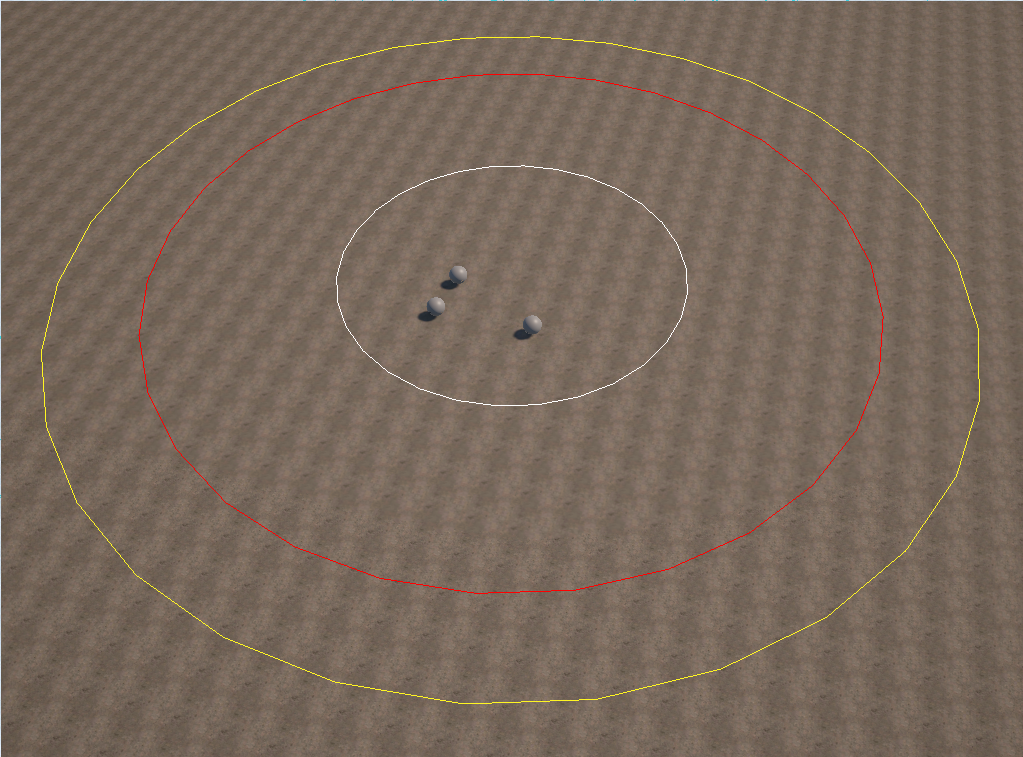
\includegraphics[width=0.6\textwidth]{images/ai}
\caption{Obraz przedstawia zasięgi odpowiednich regionów.}
\end{figure}
